% *********************************************************************
% © 2010–2022 Jeremy Sylvestre
%
% Permission is granted to copy, distribute and/or modify this document
% under the terms of the GNU Free Documentation License, Version 1.3 or
% any later version published by the Free Software Foundation; with no
% Invariant Sections, no Front-Cover Texts, and no Back-Cover Texts. A
% copy of the license is included in the appendix entitled “GNU Free
% Documentation License” that appears in the output document of this
% PreTeXt source code. All trademarks™ are the registered® marks of
% their respective owners.
%
% *********************************************************************

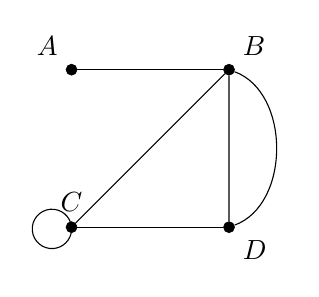
\begin{tikzpicture}[
	vertex/.style={ circle, draw, very thin, fill, inner sep=0pt, minimum size=4pt },
	vertexg/.style={ black!40!white, circle, draw, very thin, fill, inner sep=0pt, minimum size=4pt },
	vertexo/.style={ circle, draw, very thin, inner sep=0pt, minimum size=4pt }
]

\node at (0,0) (C) [vertex,label=above:$C$] {};
\node at (2,0) (D) [vertex,label=below right:$D$] {};
\node at (2,2) (B) [vertex,label=above right:$B$] {};
\node at (0,2) (A) [vertex,label=above left:$A$] {};
\draw (C) arc (5:355:0.25cm) to (C);
\foreach \p in {B,D} \draw (C) to (\p);
\draw (B) to (A);
\draw (D) to (B) to [out=-20,in=20] (D);

\end{tikzpicture}
